\documentclass[
  shownotes,
  xcolor={svgnames},
  hyperref={colorlinks,citecolor=DarkBlue,linkcolor=DarkRed,urlcolor=DarkBlue}
  , aspectratio=169]{beamer}
\usepackage{animate}
\usepackage{amsmath}
\usepackage{amsfonts}
\usepackage{amssymb}
\usepackage{pifont}
\usepackage{mathpazo}
%\usepackage{xcolor}
\usepackage{multimedia}
\usepackage{fancybox}
\usepackage[para]{threeparttable}
\usepackage{multirow}
\setcounter{MaxMatrixCols}{30}
\usepackage{subcaption}
\usepackage{graphicx}
\usepackage{lscape}
\usepackage[compatibility=false,font=small]{caption}
\usepackage{booktabs}
\usepackage{ragged2e}
\usepackage{chronosys}
\usepackage{appendixnumberbeamer}
\usepackage{animate}
\setbeamertemplate{caption}[numbered]
\usepackage{color}
%\usepackage{times}
\usepackage{tikz}
\usepackage{comment} %to comment
%% BibTeX settings
\usepackage{natbib}
\bibliographystyle{apalike}
\bibpunct{(}{)}{,}{a}{,}{,}
\setbeamertemplate{bibliography item}{[\theenumiv]}

% Defines columns for bespoke tables
\usepackage{array}
\newcolumntype{L}[1]{>{\raggedright\let\newline\\\arraybackslash\hspace{0pt}}m{#1}}
\newcolumntype{C}[1]{>{\centering\let\newline\\\arraybackslash\hspace{0pt}}m{#1}}
\newcolumntype{R}[1]{>{\raggedleft\let\newline\\\arraybackslash\hspace{0pt}}m{#1}}


\usepackage{xfrac}


\usepackage{multicol}
\setlength{\columnsep}{0.5cm}

% Theme and colors
\usetheme{Boadilla}

% I use steel blue and a custom color palette. This defines it.
\definecolor{andesred}{HTML}{af2433}

% Other options
\providecommand{\U}[1]{\protect\rule{.1in}{.1in}}
\usefonttheme{serif}
\setbeamertemplate{itemize items}[default]
\setbeamertemplate{enumerate items}[square]
\setbeamertemplate{section in toc}[circle]

\makeatletter

\definecolor{mybackground}{HTML}{82CAFA}
\definecolor{myforeground}{HTML}{0000A0}

\setbeamercolor{normal text}{fg=black,bg=white}
\setbeamercolor{alerted text}{fg=red}
\setbeamercolor{example text}{fg=black}

\setbeamercolor{background canvas}{fg=myforeground, bg=white}
\setbeamercolor{background}{fg=myforeground, bg=mybackground}

\setbeamercolor{palette primary}{fg=black, bg=gray!30!white}
\setbeamercolor{palette secondary}{fg=black, bg=gray!20!white}
\setbeamercolor{palette tertiary}{fg=white, bg=andesred}

\setbeamercolor{frametitle}{fg=andesred}
\setbeamercolor{title}{fg=andesred}
\setbeamercolor{block title}{fg=andesred}
\setbeamercolor{itemize item}{fg=andesred}
\setbeamercolor{itemize subitem}{fg=andesred}
\setbeamercolor{itemize subsubitem}{fg=andesred}
\setbeamercolor{enumerate item}{fg=andesred}
\setbeamercolor{item projected}{bg=gray!30!white,fg=andesred}
\setbeamercolor{enumerate subitem}{fg=andesred}
\setbeamercolor{section number projected}{bg=gray!30!white,fg=andesred}
\setbeamercolor{section in toc}{fg=andesred}
\setbeamercolor{caption name}{fg=andesred}
\setbeamercolor{button}{bg=gray!30!white,fg=andesred}


\usepackage{fancyvrb}
\newcommand{\VerbBar}{|}
\newcommand{\VERB}{\Verb[commandchars=\\\{\}]}
\DefineVerbatimEnvironment{Highlighting}{Verbatim}{commandchars=\\\{\}}
% Add ',fontsize=\small' for more characters per line
\usepackage{framed}
\definecolor{shadecolor}{RGB}{248,248,248}
\newenvironment{Shaded}{\begin{snugshade}}{\end{snugshade}}
\newcommand{\AlertTok}[1]{\textcolor[rgb]{0.94,0.16,0.16}{#1}}
\newcommand{\AnnotationTok}[1]{\textcolor[rgb]{0.56,0.35,0.01}{\textbf{\textit{#1}}}}
\newcommand{\AttributeTok}[1]{\textcolor[rgb]{0.77,0.63,0.00}{#1}}
\newcommand{\BaseNTok}[1]{\textcolor[rgb]{0.00,0.00,0.81}{#1}}
\newcommand{\BuiltInTok}[1]{#1}
\newcommand{\CharTok}[1]{\textcolor[rgb]{0.31,0.60,0.02}{#1}}
\newcommand{\CommentTok}[1]{\textcolor[rgb]{0.56,0.35,0.01}{\textit{#1}}}
\newcommand{\CommentVarTok}[1]{\textcolor[rgb]{0.56,0.35,0.01}{\textbf{\textit{#1}}}}
\newcommand{\ConstantTok}[1]{\textcolor[rgb]{0.00,0.00,0.00}{#1}}
\newcommand{\ControlFlowTok}[1]{\textcolor[rgb]{0.13,0.29,0.53}{\textbf{#1}}}
\newcommand{\DataTypeTok}[1]{\textcolor[rgb]{0.13,0.29,0.53}{#1}}
\newcommand{\DecValTok}[1]{\textcolor[rgb]{0.00,0.00,0.81}{#1}}
\newcommand{\DocumentationTok}[1]{\textcolor[rgb]{0.56,0.35,0.01}{\textbf{\textit{#1}}}}
\newcommand{\ErrorTok}[1]{\textcolor[rgb]{0.64,0.00,0.00}{\textbf{#1}}}
\newcommand{\ExtensionTok}[1]{#1}
\newcommand{\FloatTok}[1]{\textcolor[rgb]{0.00,0.00,0.81}{#1}}
\newcommand{\FunctionTok}[1]{\textcolor[rgb]{0.00,0.00,0.00}{#1}}
\newcommand{\ImportTok}[1]{#1}
\newcommand{\InformationTok}[1]{\textcolor[rgb]{0.56,0.35,0.01}{\textbf{\textit{#1}}}}
\newcommand{\KeywordTok}[1]{\textcolor[rgb]{0.13,0.29,0.53}{\textbf{#1}}}
\newcommand{\NormalTok}[1]{#1}
\newcommand{\OperatorTok}[1]{\textcolor[rgb]{0.81,0.36,0.00}{\textbf{#1}}}
\newcommand{\OtherTok}[1]{\textcolor[rgb]{0.56,0.35,0.01}{#1}}
\newcommand{\PreprocessorTok}[1]{\textcolor[rgb]{0.56,0.35,0.01}{\textit{#1}}}
\newcommand{\RegionMarkerTok}[1]{#1}
\newcommand{\SpecialCharTok}[1]{\textcolor[rgb]{0.00,0.00,0.00}{#1}}
\newcommand{\SpecialStringTok}[1]{\textcolor[rgb]{0.31,0.60,0.02}{#1}}
\newcommand{\StringTok}[1]{\textcolor[rgb]{0.31,0.60,0.02}{#1}}
\newcommand{\VariableTok}[1]{\textcolor[rgb]{0.00,0.00,0.00}{#1}}
\newcommand{\VerbatimStringTok}[1]{\textcolor[rgb]{0.31,0.60,0.02}{#1}}
\newcommand{\WarningTok}[1]{\textcolor[rgb]{0.56,0.35,0.01}{\textbf{\textit{#1}}}}
\usepackage{graphicx}
\makeatletter

\definecolor{airforceblue}{rgb}{0.36, 0.54, 0.66}

\usepackage{tikz}
% Tikz settings optimized for causal graphs.
\usetikzlibrary{shapes,decorations,arrows,calc,arrows.meta,fit,positioning}
\tikzset{
    -Latex,auto,node distance =1 cm and 1 cm,semithick,
    state/.style ={ellipse, draw, minimum width = 0.7 cm},
    point/.style = {circle, draw, inner sep=0.04cm,fill,node contents={}},
    bidirected/.style={Latex-Latex,dashed},
    el/.style = {inner sep=2pt, align=left, sloped}
}


\makeatother






%%%%%%%%%%%%%%% BEGINS DOCUMENT %%%%%%%%%%%%%%%%%%

\begin{document}
 
\title[Lecture 17]{Lecture 17: \\ Regularization/Shrinkage Methods- Elastic Net  \\ Classification}
\subtitle{Big Data and Machine Learning for Applied Economics \\ Econ 4676}
\date{\today}

\author[Sarmiento-Barbieri]{Ignacio Sarmiento-Barbieri}
\institute[Uniandes]{Universidad de los Andes}


\begin{frame}[noframenumbering]
\maketitle
\end{frame}

%%%%%%%%%%%%%%%%%%%%%%%%%%%%%%%%%%%



%----------------------------------------------------------------------% 

\begin{frame}
\frametitle{Agenda}

\tableofcontents

\end{frame}

%----------------------------------------------------------------------%
\section{Recap }
\subsection{Lasso}
%----------------------------------------------------------------------%
\begin{frame}[fragile]
\frametitle{Overfit and out of Sample Prediction}

\frametitle{Demo Regularization}

   \begin{figure}[H] \centering
            \captionsetup{justification=centering}
              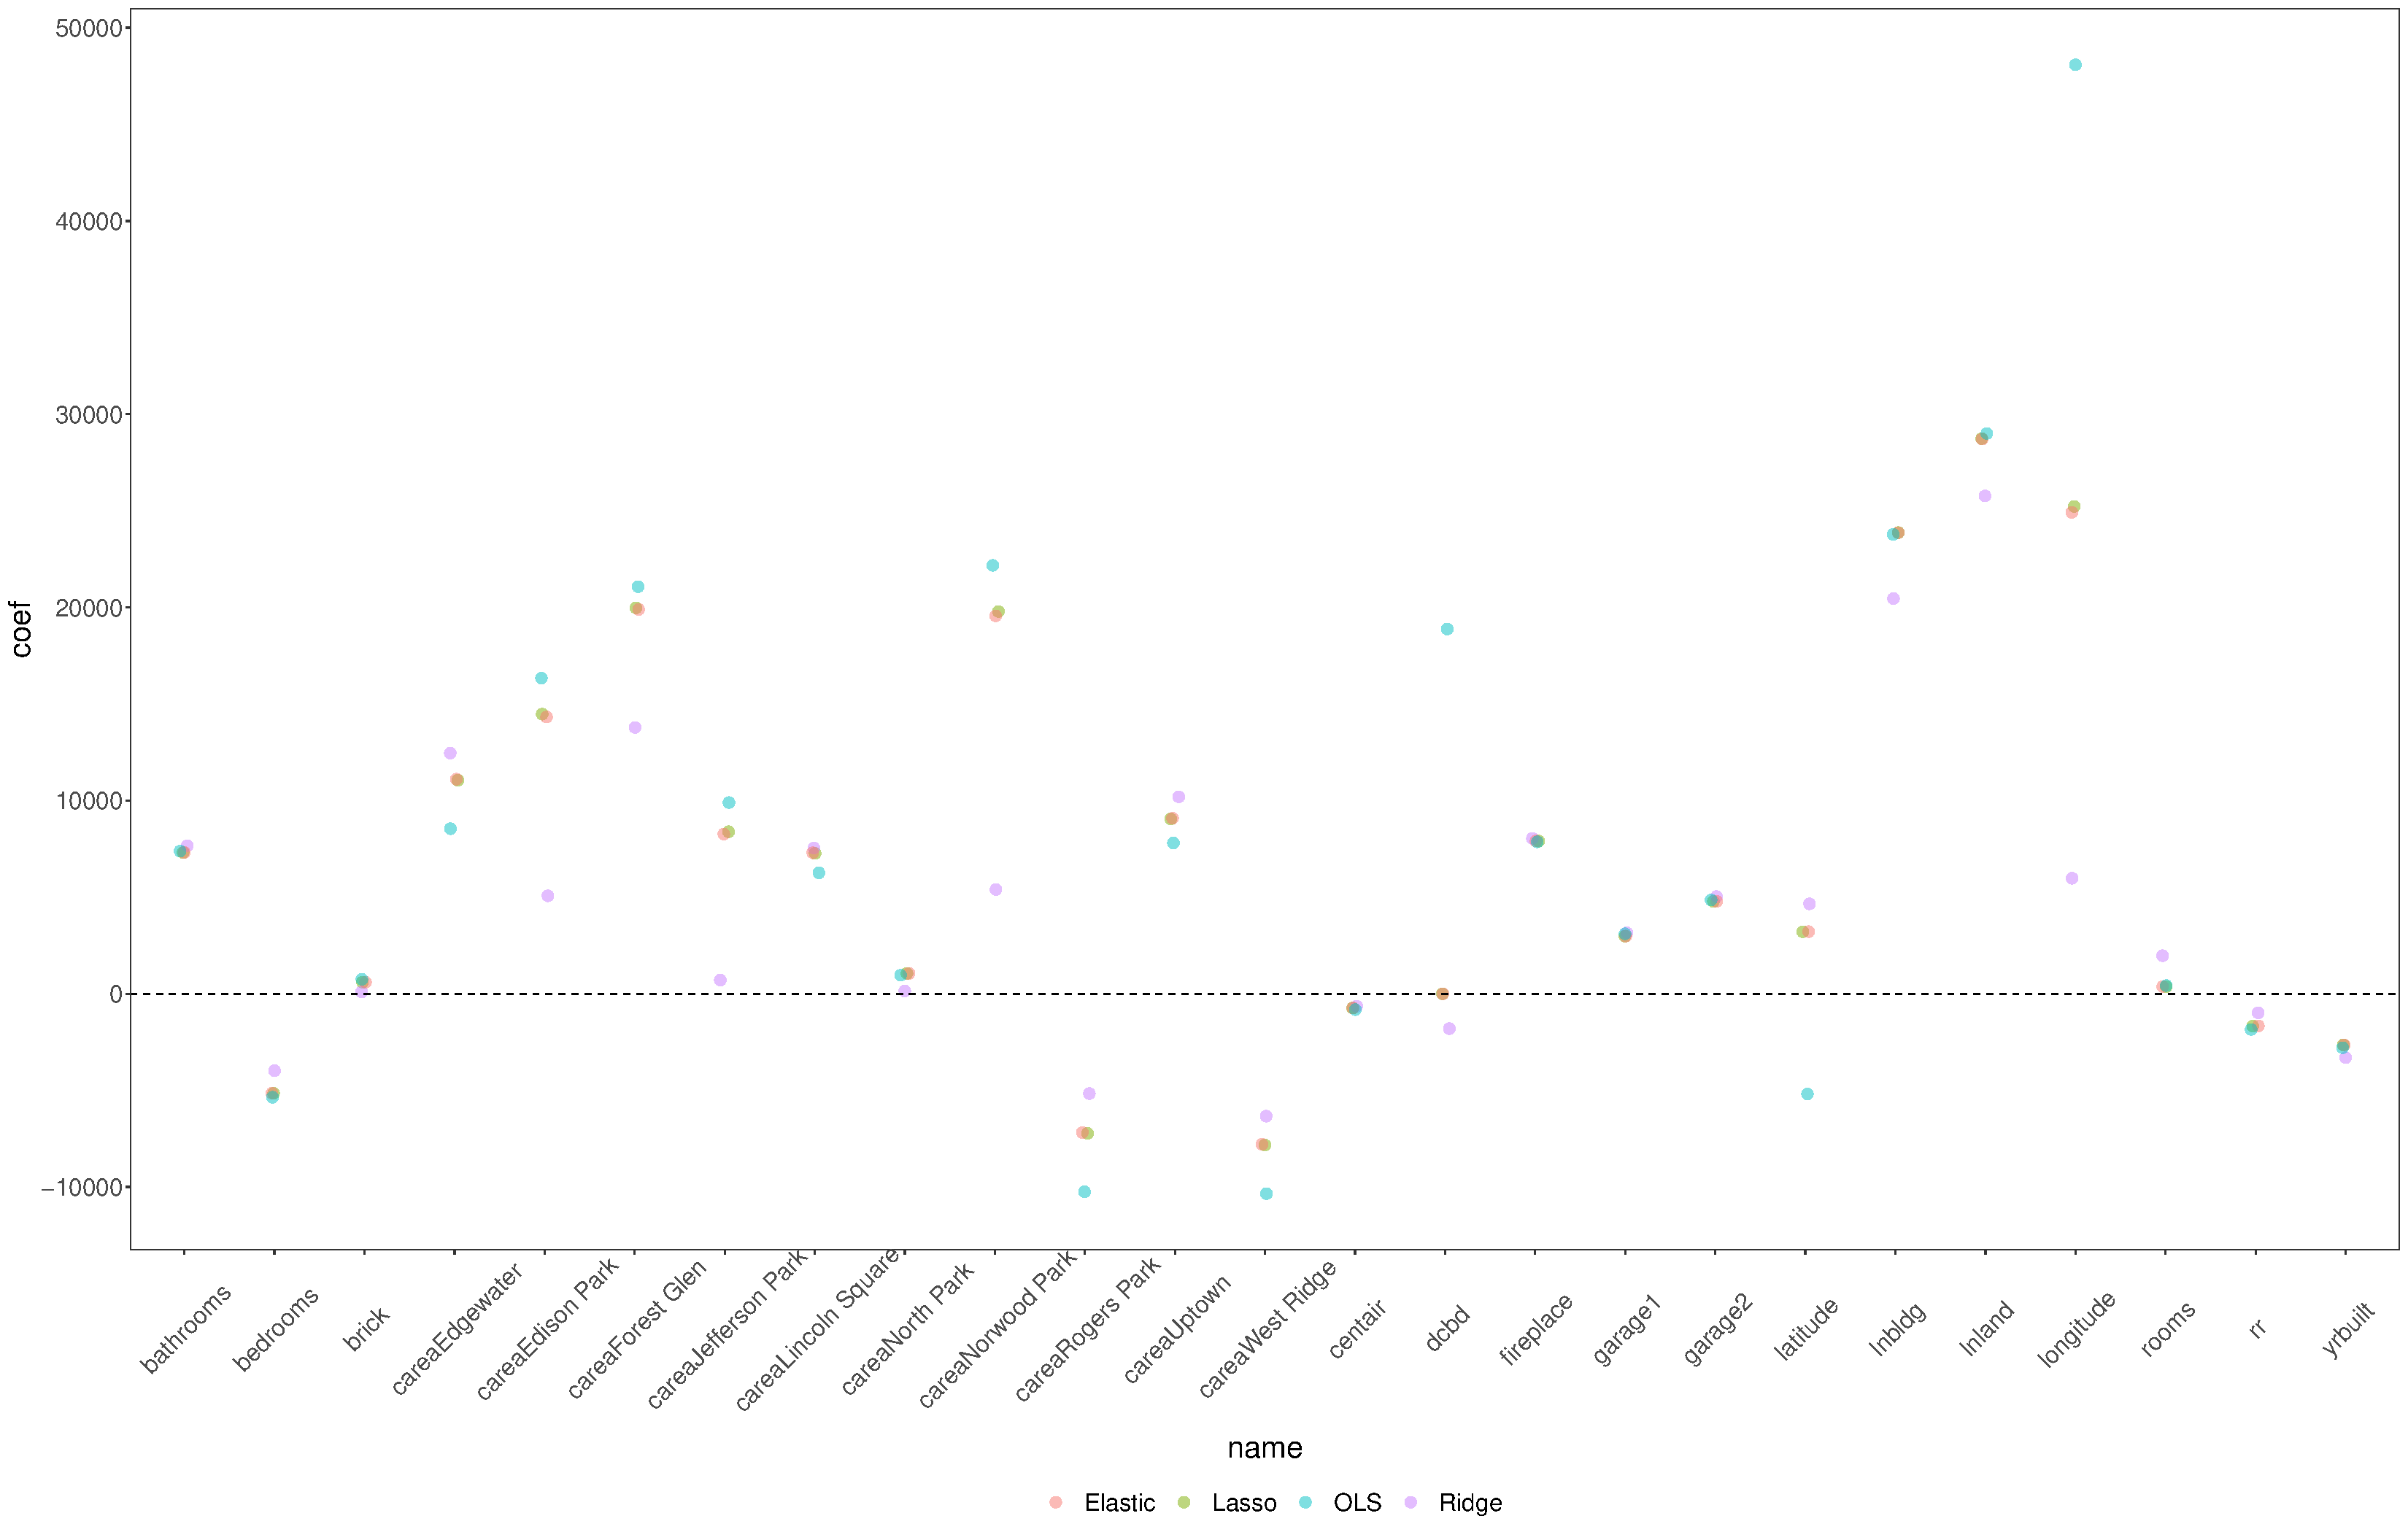
\includegraphics[scale=0.2]{figures/comp}
 \end{figure}


\end{frame}
%----------------------------------------------------------------------%
\begin{frame}[fragile]
\frametitle{Motivation}

\begin{itemize}
  \item Accuracy: Minimize prediction error (in one step) $\rightarrow$ Ridge, Lasso
  \item Dimentionality: reduce the predictor space $\rightarrow$ Lasso's free lunch
\end{itemize}
\bigskip
\begin{itemize}
  \item What happens when we have $k>n$?
  \begin{itemize}
   \item OLS fails
   \item Ridge and Lasso to the rescue?
  \end{itemize}
\end{itemize}

\end{frame}

%----------------------------------------------------------------------%
\begin{frame}[fragile]
\frametitle{Prediction}

\begin{itemize}
  \item Rank? Max number of rows or columns that are linearly independent
  \item MCO we need $rank(X_{k\times n}) \leq min(k,n)$. Why?)
  \item If $rank(X_{k\times n})=k$ then $rank(X'X)=k$
  \item So if $k>n$, then  $rank(X'X)\leq n < k$ then $X'X$ cannot be inverted
  \item Ridge and Lasso work when $k \geq n$
\end{itemize}

\end{frame}

%----------------------------------------------------------------------%
\begin{frame}[fragile]
\frametitle{Ridge when $k>n$}


\begin{itemize}
  \item Solution $\rightarrow$ data augmentation
  \item Problem set 2 HW
  \item Intuition: Ridge ``adds'' $k$ additional points.
  \item Allows us to ``deal'' with $k\geq n$
\end{itemize}

\end{frame}
%----------------------------------------------------------------------%
\begin{frame}[fragile]
\frametitle{Problems with Lasso}

\begin{itemize}
\item When $k>n$ chooses at most $k$ variables
\item When we have a group of highly correlated variables, it tends to choose only one. Arbitrarily!!!
\item Makes it unstable fro prediction. (Doesn't happen to Ridge)
\item When $k>n$ and there's high correlation among predictors, Ridge tends to ``work'' better than Lasso. ``Work'' in terms of prediction error
\item Elastic net: happy medium. Predicts well, reduces dimensionality, selects well variables
\end{itemize}



\end{frame}
%----------------------------------------------------------------------%
\begin{frame}[fragile]
\frametitle{Problems with Lasso}



\begin{align}
min_{\beta} EL(\beta) &= \sum_{i=1}^n (y_i-x_i'\beta)^2 + \lambda_1 \sum_{s=2}^p |\beta_s| + \lambda_2 \sum_{s=2}^p \beta_s^2 \nonumber \\
 &= \sum_{i=1}^n (y_i-x_i'\beta)^2 + \lambda \sum_{s=2}^p \left(  (1-\alpha) \beta_s^2 + \alpha  |\beta_s|\right)
\end{align}


\begin{itemize}
 \item Mixes Ridge and Lasso
 \item Lasso selects predictors
 \item Strict convexity part  of the penalty (ridge) solve the grouping instability problem 
\end{itemize}


\end{frame}
%----------------------------------------------------------------------%
\begin{frame}[fragile]
\frametitle{Problems with Lasso}

Let $\beta_{OLS}>0$ one predictor standarized

\begin{align}
\hat{\beta}_{naive\,EN}= \frac{\left(\hat{\beta}_{OLS}-\frac{\lambda_1}{2}\right)_{+}}{1+\lambda_2}
\end{align}

\begin{itemize}
\item Where $+$ refers to the positive part, e.g. $(x)_{+}$ takes $x$ if $x>0$ and $0$ otherwise
\end{itemize}

\end{frame}
%----------------------------------------------------------------------%
\begin{frame}[fragile]
\frametitle{Reescaled version}


\begin{align}
\hat{\beta}_{EN}= \frac{\hat{\beta}_{naive\,EN}}{\sqrt{1+\lambda_2}}
\end{align}

\begin{itemize}
\item How to choose $(\lambda_1,\lambda_2)$?
\item Bidimensional Crossvalidation
\end{itemize}

\end{frame}

%----------------------------------------------------------------------%
\section{Classification}
%----------------------------------------------------------------------%
\begin{frame}[fragile]
\frametitle{Classification}


\centering
{\huge \textcolor{andesred}{Classification}}



\end{frame}
%----------------------------------------------------------------------%
\begin{frame}[fragile]
\frametitle{Motivation}

\begin{itemize}
\item Admit a student to $PEG$ based on their grades and lor
\item Give a credit, based on credit history, demographics?
\item Classifying emails: spam, personal, social based on email contents
\bigskip
\item Aim is to classify $y$ based on $X's$
\item $y$ is
\begin{itemize}
  \item qualitative (e.g., spam, personal, social)
  \item Not necessarily ordered
  \item Not necessarily two categories, but will start with the binary case

\end{itemize}
\end{itemize}


\end{frame}
%----------------------------------------------------------------------%
\begin{frame}[fragile]
\frametitle{Motivation}

\begin{itemize}
  \item Two states of nature $y=\{0,1\}$
  \item Two actions $\hat{y}=\{0,1\}$
\end{itemize}

\begin{table}[H]
\centering
\begin{tabular}{cccc}
 & \multicolumn{3}{c}{$y$}\tabularnewline
 &  & 0 & 1 \\
 \hline
\multirow{2}{*}{$\hat{y}$} & 0 & True Negative & False Negative \\
 & 1 & False Positive & True Negative \\
\end{tabular}
\end{table}






\end{frame}
%----------------------------------------------------------------------%
\section{Review}
%----------------------------------------------------------------------%
\begin{frame}[fragile]
\frametitle{Review}

   

 \end{frame}
%----------------------------------------------------------------------%
\section{Further Readings}
%----------------------------------------------------------------------%
\begin{frame}
\frametitle{Further Readings}

\begin{itemize}


  \item Friedman, J., Hastie, T., \& Tibshirani, R. (2001). The elements of statistical learning (Vol. 1, No. 10). New York: Springer series in statistics.
  \medskip
  \item James, G., Witten, D., Hastie, T., \& Tibshirani, R. (2013). An introduction to statistical learning (Vol. 112, p. 18). New York: springer.
  \medskip
  \item Kuhn, M. (2012). The caret package. R Foundation for Statistical Computing, Vienna, Austria. \url{https://topepo.github.io/caret/index.html}
  \medskip
  \item Taddy, M. (2019). Business data science: Combining machine learning and economics to optimize, automate, and accelerate business decisions. McGraw Hill Professional.
  \medskip
  \item  Zou, H. y Hastie, T., 2005, Regularization and variable selection via the elastic net, Journal of the Royal Statistical Society, 67, 2, 301-320.
  
\end{itemize}

\end{frame}






%----------------------------------------------------------------------%
%----------------------------------------------------------------------%
\end{document}
%----------------------------------------------------------------------%
%----------------------------------------------------------------------%

